%*******************************************************************************
%****************************** Fifth Chapter *********************************
%*******************************************************************************

\chapter{Cosmic Muon Tomography}

\ifpdf
    \graphicspath{{Chapter5/Figs/Raster/}{Chapter5/Figs/PDF/}{Chapter5/Figs/}}
\else
    \graphicspath{{Chapter5/Figs/Vector/}{Chapter5/Figs/}}
\fi

\section{Deployment At Wylfa}\label{sec:deploymentAtWylfa}
The original prototype detector was deployed at the Wylfa Nuclear power station from 07-07-2014 to 25-02-2016 with data being taken continuously over that time period both with the reactor on and off with ibd measurements seen in figure \ref{fig:prototypeMeasumentFlux}. The placement of the detector in relation to the Wylfa reactor buildings can be seen in figure \ref{fig:wylfaTrace} the reactors were placed either end of the main reactor building in the centre of the cylindrical shaped ends. The overall shape of each of these buildings seen in figure \ref{fig:wylfaAir} causes the shape of the shadow to be quite different from what might be expected. The overall shadow in both $\theta$ and $\phi$ will therefore be an overlapping series of boxes rather than just one.   
 
\begin{figure}[H]
 \centering
 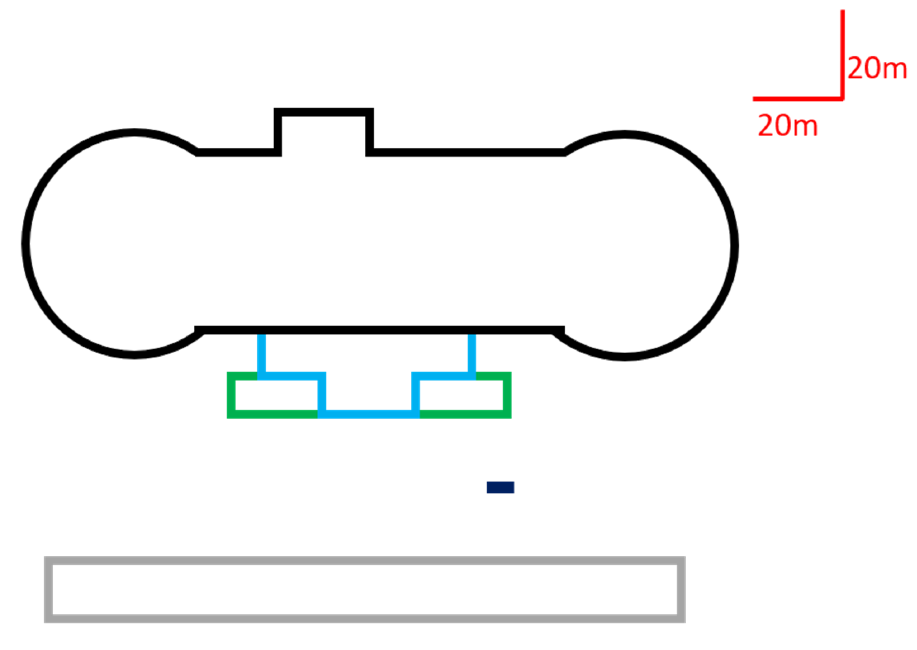
\includegraphics[width=0.7\linewidth]{Chapter5/Figs/Raster/wylfaTrace.png}
 \captionof{figure}{The position of the detector (dark blue) shown to scale compared with the main reactor building (black) with the secondary reactor buildings shown (cyan and green) which are of differing heights. The turbine hall (grey) is behind the detector. \hl{position of detector may be slightly off check with George}} %~can be used as a kind of place holder in latex
 \label{fig:wylfaTrace}
\end{figure}

\begin{figure}[H]
 \centering
 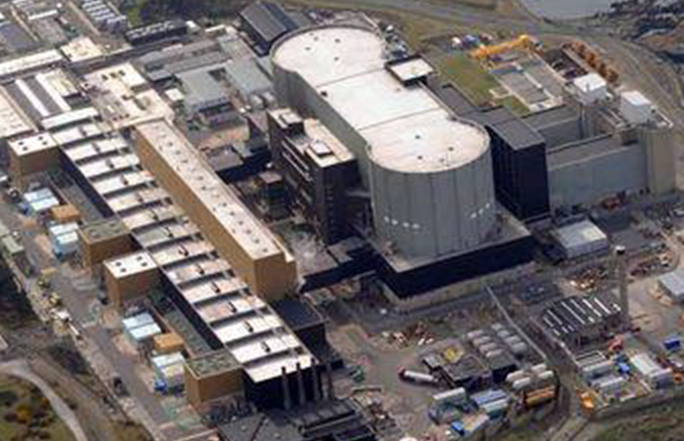
\includegraphics[width=0.7\linewidth]{Chapter5/Figs/Raster/wylfaArielView.png}
 \captionof{figure}{An aerial view of the Wylfa power station the main reactor building is the the shape of a "dog bone" the detector was placed in-between the turbine hall and reactor building.} %~can be used as a kind of place holder in latex
 \label{fig:wylfaAir}
\end{figure}


\section{Reactor Shadow} \label{sec:ReactorShadow}
When measuring $\theta$ and $\phi$ the reactor and turbine hall should block some of the cosmic rays which should then be measurable 

\begin{figure}[H]
 \centering
 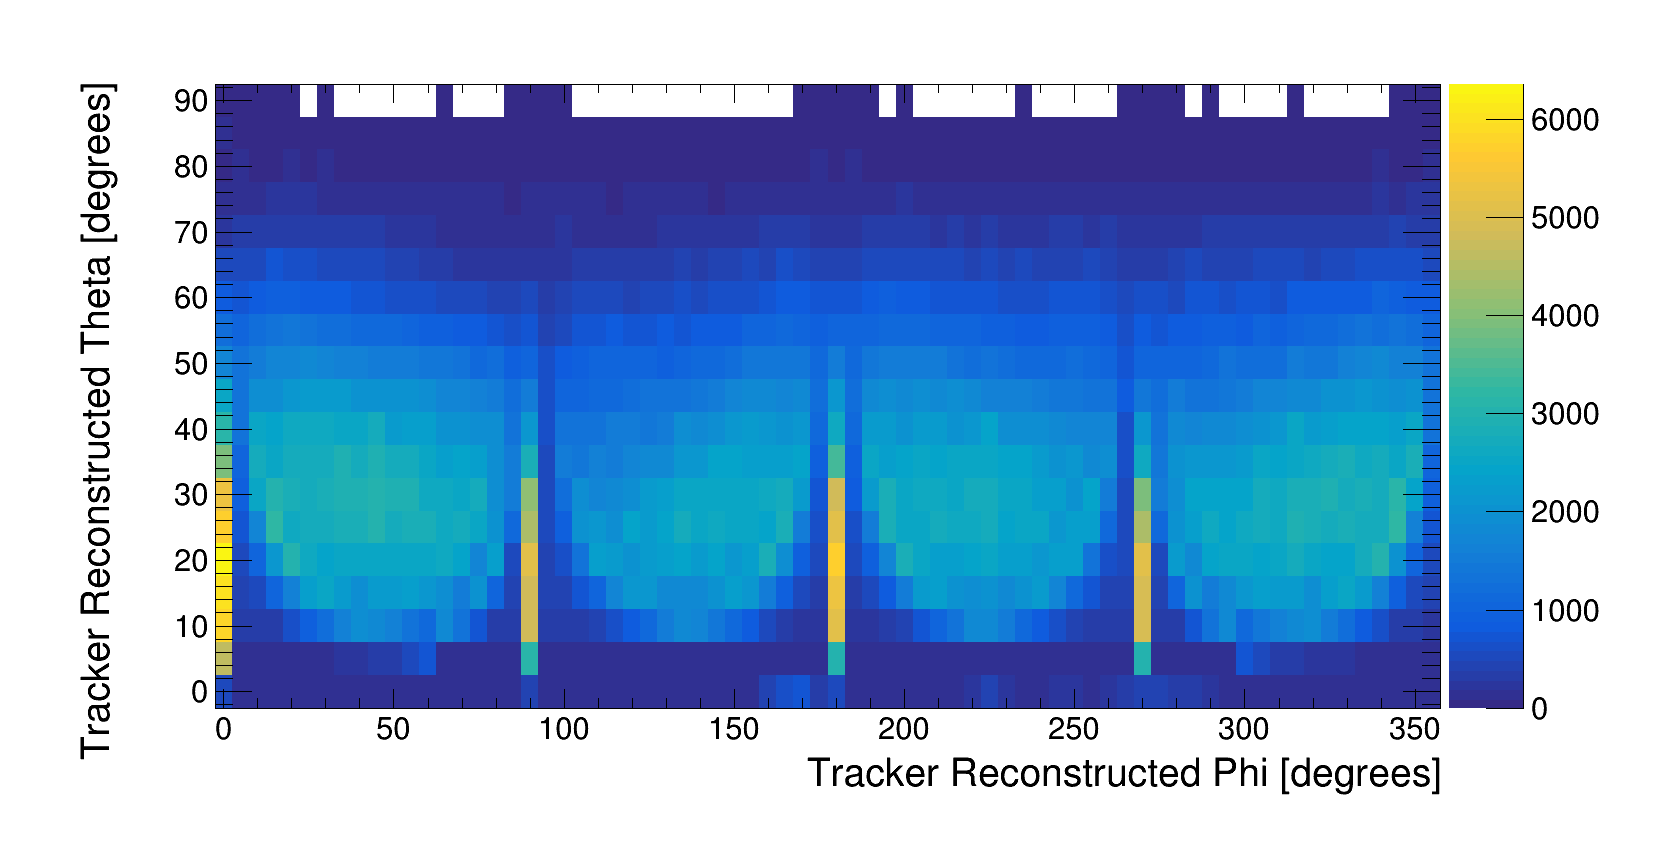
\includegraphics[width=0.8\linewidth]{Chapter5/Figs/Raster/simpleTrackTheta3000-9999IncBelow10.png}
 \captionof{figure}{Measured $\theta$ and $\phi$ from the cosmic muons from the Wylfa deployment, the reactor is at $\sim$ 90$^{\circ}$. The turbine hall is at $\sim$ 270$^{\circ}$.} 
 \label{fig:reactorShadowSimpleTracker}
\end{figure}

\begin{figure}[H]
 \centering
 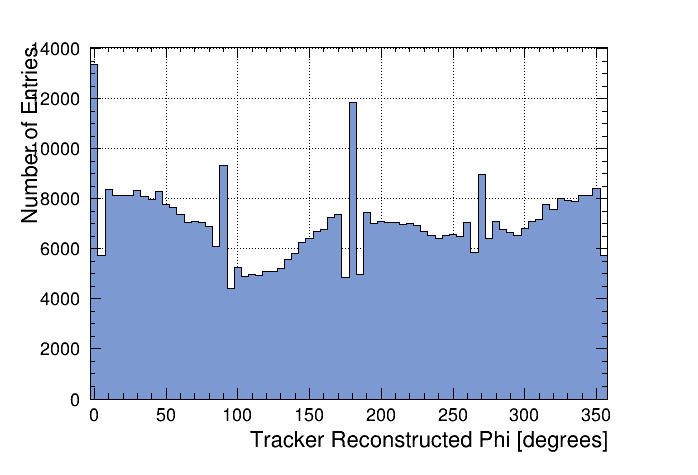
\includegraphics[width=0.8\linewidth]{Chapter5/Figs/Raster/p_realWorldAbove32.5.png}
 \captionof{figure}{Measured $\phi$ above 32.5$^{\circ}$. The reactor shadow is clearly visible between 87.5$^{\circ}$ - 142.5$^{\circ}$ The turbine hall shadow is approximated to be between 237.5$^{\circ}$ - 292.5$^{\circ}$ but it is much less clear}
 \label{fig:pRealWorldAbove52.5}
\end{figure}

\begin{figure}[H]
 \centering
 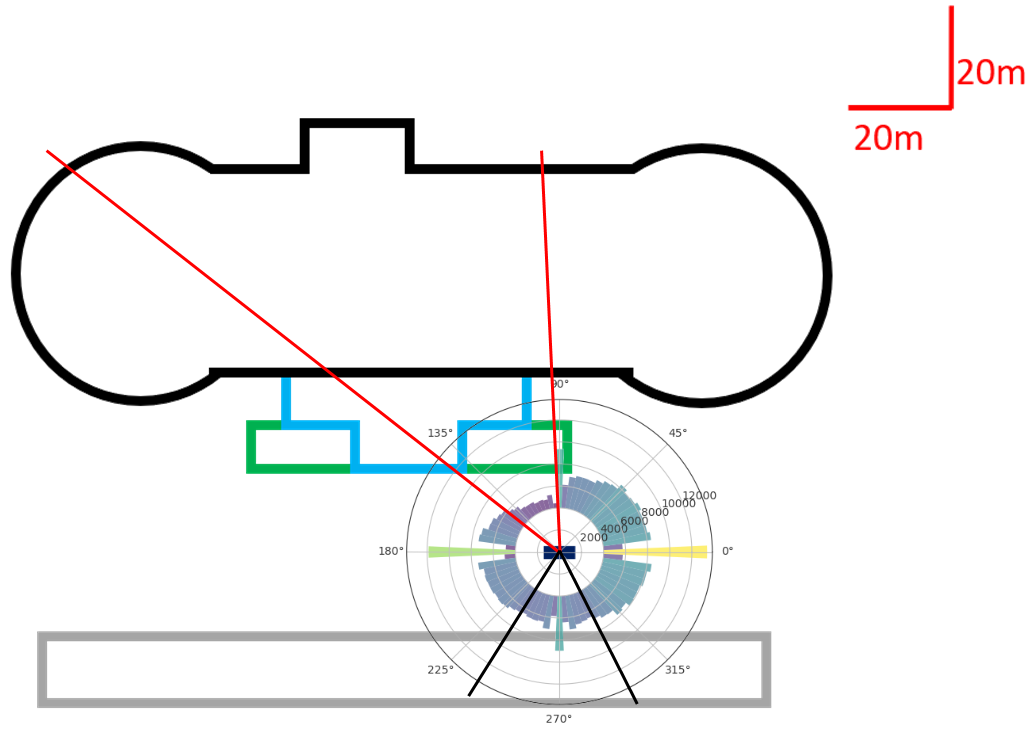
\includegraphics[width=0.8\linewidth]{Chapter5/Figs/Raster/wylfaTrace_above32.5.png}
 \captionof{figure}{The circular distribution of the $\phi$ above a $\theta$ of 32.5$^\circ$ the tower closest to the detector is dominating the distribution of the shadow.} %~can be used as a kind of place holder in latex
 \label{fig:wylfaTraceAbove32.5}
\end{figure}

\begin{figure}[H]
 \centering
 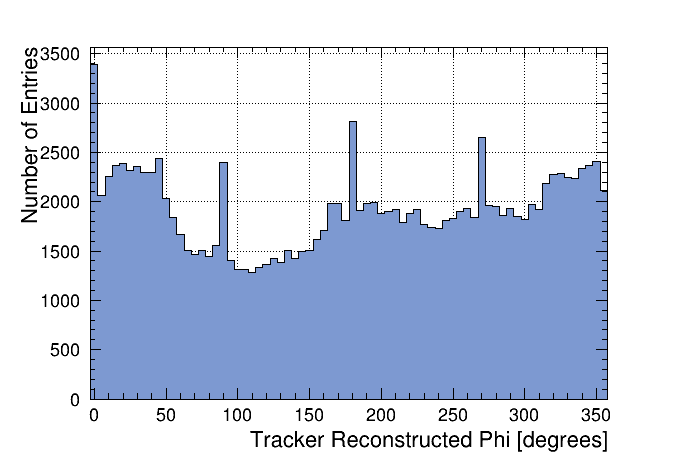
\includegraphics[width=0.8\linewidth]{Chapter5/Figs/Raster/p_realWorldAbove52.5.png}
 \captionof{figure}{Measured $\phi$ above 52.5$^{\circ}$. The reactor shadow is clearly visible between 162.5$^{\circ}$-47.5$^{\circ}$ and the turbine hall is approximated to be between $\sim$ 197.5$^{\circ}$ - 312.5$^{\circ}$ } 
 \label{fig:pRealWorldAbove52.5}
\end{figure}

\begin{figure}[H]
 \centering
 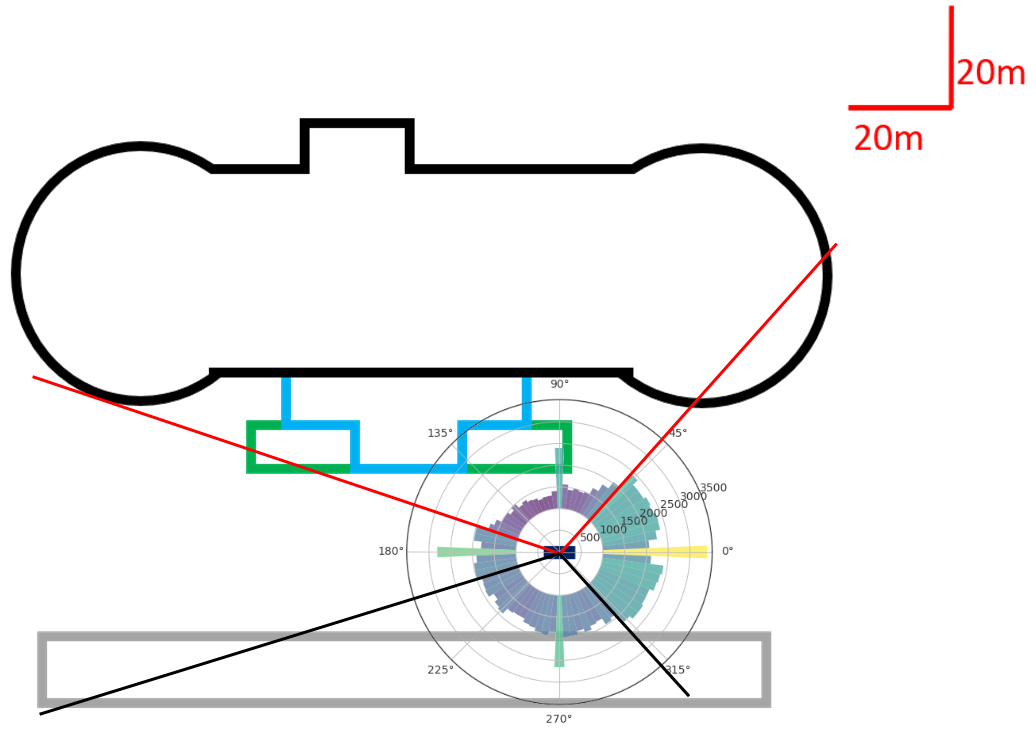
\includegraphics[width=0.8\linewidth]{Chapter5/Figs/Raster/wylfaTrace_above52.5.png}
 \captionof{figure}{The circular distribution of the $\phi$ above a $\theta$ of 52.5$^\circ$ the reactor shadow is now dominated by the main reactor building } %~can be used as a kind of place holder in latex
 \label{fig:wylfaTraceAbove52.5}
\end{figure}

\begin{figure}[H]
 \centering
 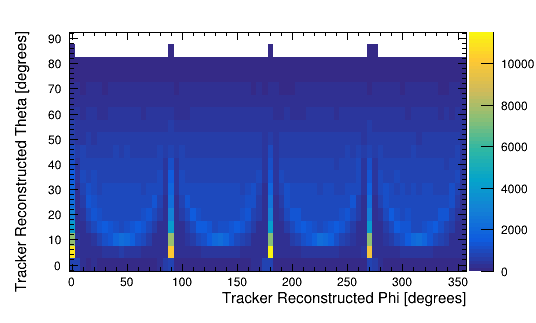
\includegraphics[width=0.8\linewidth]{Chapter5/Figs/Raster/simulatedNormalDistirbution.png}
 \captionof{figure}{Simulated distribution with an ideally generated cosmic distribution.} %~can be used as a kind of place holder in latex
 \label{fig:simulatedNormalDist}
\end{figure}

\begin{figure}[H]
 \centering
 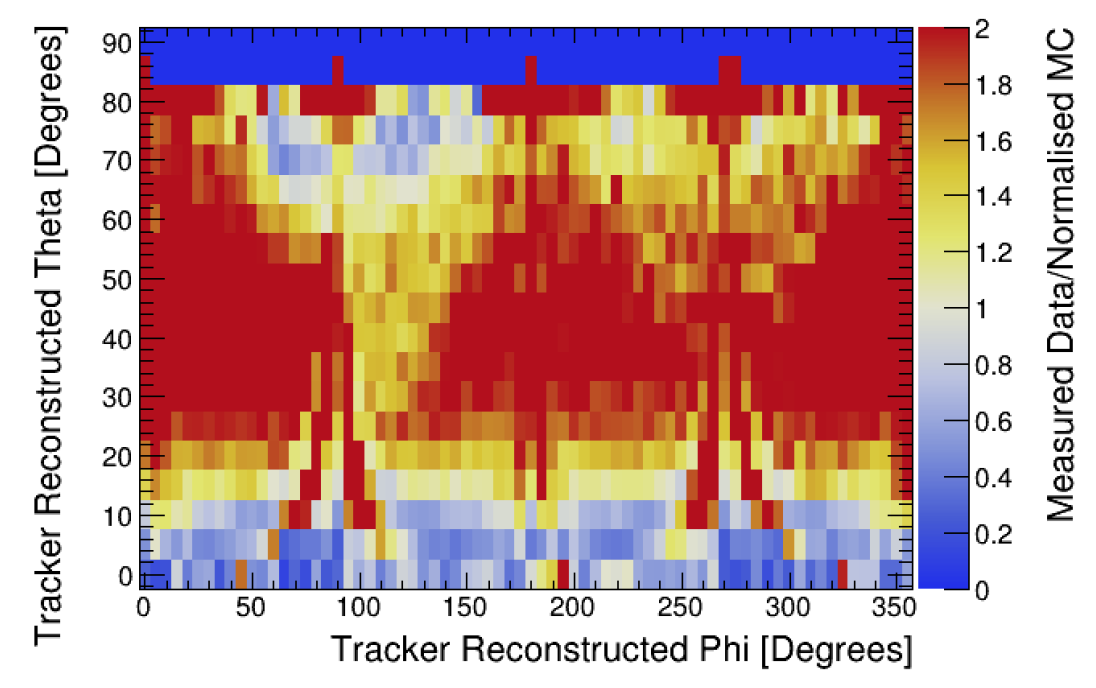
\includegraphics[width=0.8\linewidth]{Chapter5/Figs/Raster/measured_div_Simulated.png}
 \captionof{figure}{The ratio of the measured $\theta$ and $\phi$ divided by the simulated $\theta$ and $\phi$ which had the same number of events generated. The maximum allowed ratio was then limited to 2 in order to highlight the reactor shadow.} %~can be used as a kind of place holder in latex
 \label{fig:measuredDivSimulated}
\end{figure}

\begin{figure}[H]
 \centering
 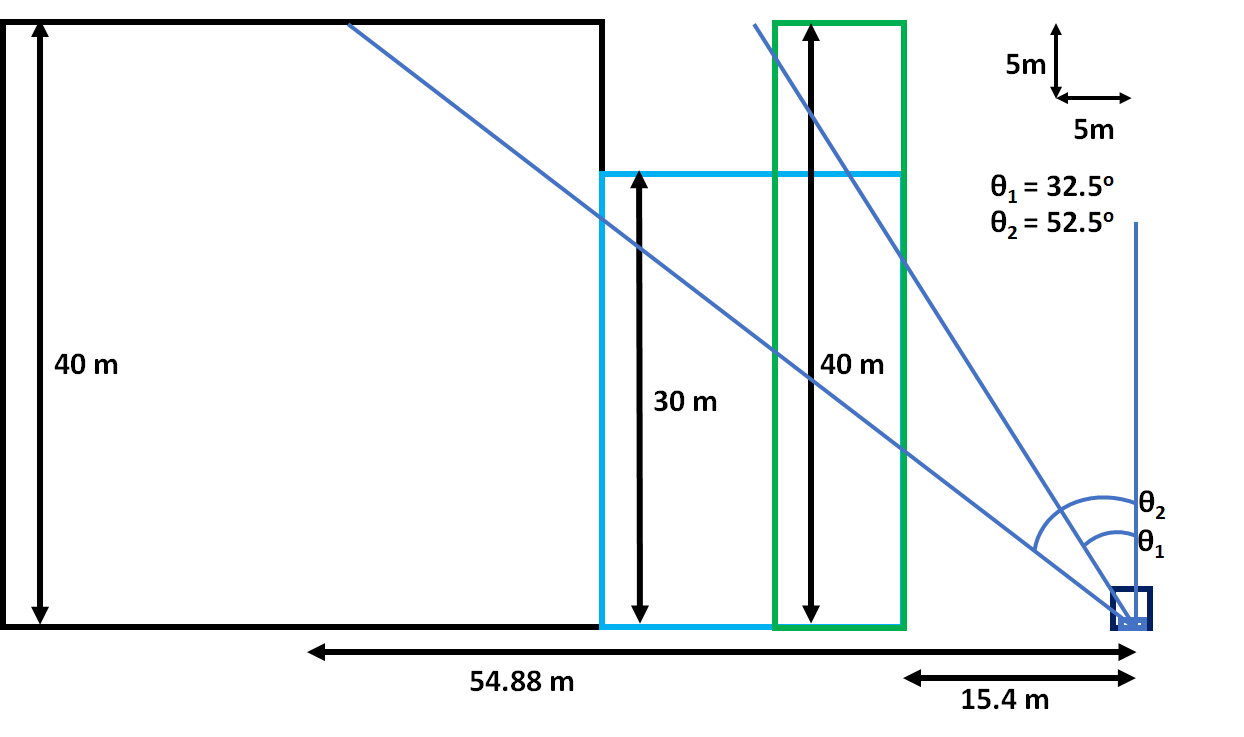
\includegraphics[width=1.0\linewidth]{Chapter5/Figs/Raster/wyflaHieghts.png}
 \captionof{figure}{The estimated heights of the reactor buildings, above 32.5$^{\circ}$ the green tower closest to the detector dominates, above 52.5$^{\circ}$ the main reactor building dominates the shadow.} %~can be used as a kind of place holder in latex
 \label{fig:wylfaHieghts}
\end{figure}


\begin{figure}[H]
 \centering
 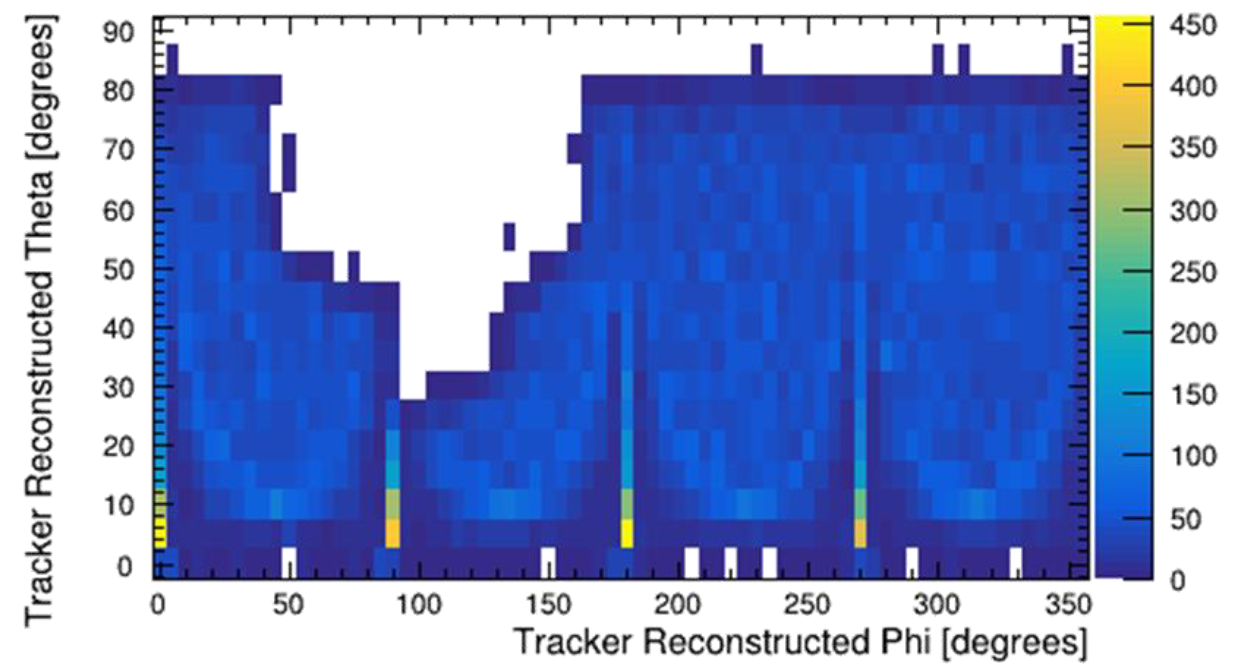
\includegraphics[width=0.8\linewidth]{Chapter5/Figs/Raster/simulatedShadowDistribution.png}
 \captionof{figure}{The simulated reactor shadow assuming the heights calculated from figures \ref{fig:measuredDivSimulated} and \ref{fig:wylfaHieghts}} %~can be used as a kind of place holder in latex
 \label{fig:simulatedShadowDist}
\end{figure}


% end